\chapter{Implementazione}
    In questo capitolo si presenterà il codice generato da Matlab, esportato tramite l'add-on Embedded Coder ed il successivo caricamento del firmware sulla scheda STM32 Nucleo  G474RE.

    \section{Realizzazione del circuito}
        \noindent I componenti utilizzati per realizzare il circuito sono i seguenti:
        
        \begin{table}[H]
            \centering
                \begin{tabular}{ | c | c | c | c |} 
                    \hline
                            
                    \textbf{Componente} & \textbf{Pin} \\ 
                    \hline
                            
                    B1 & PC8\\ 
                    \hline
                            
                    B2 & PC6\\ 
                    \hline

                    B3 & PC5\\ 
                    \hline

                    P1 & PC2\\ 
                    \hline

                    P2 & PC3\\ 
                    \hline

                    LedG & PB5\\ 
                    \hline

                    LedY & PB4\\ 
                    \hline

                    LedR & PB3\\ 
                    \hline
                \end{tabular}
            \caption{Tabella variabili Tuning}
        \end{table}

        \noindent In figura \ref{sketch} è presente il circuito realizzato sul software Fritzing.

        \begin{figure}[H]
            \centering
            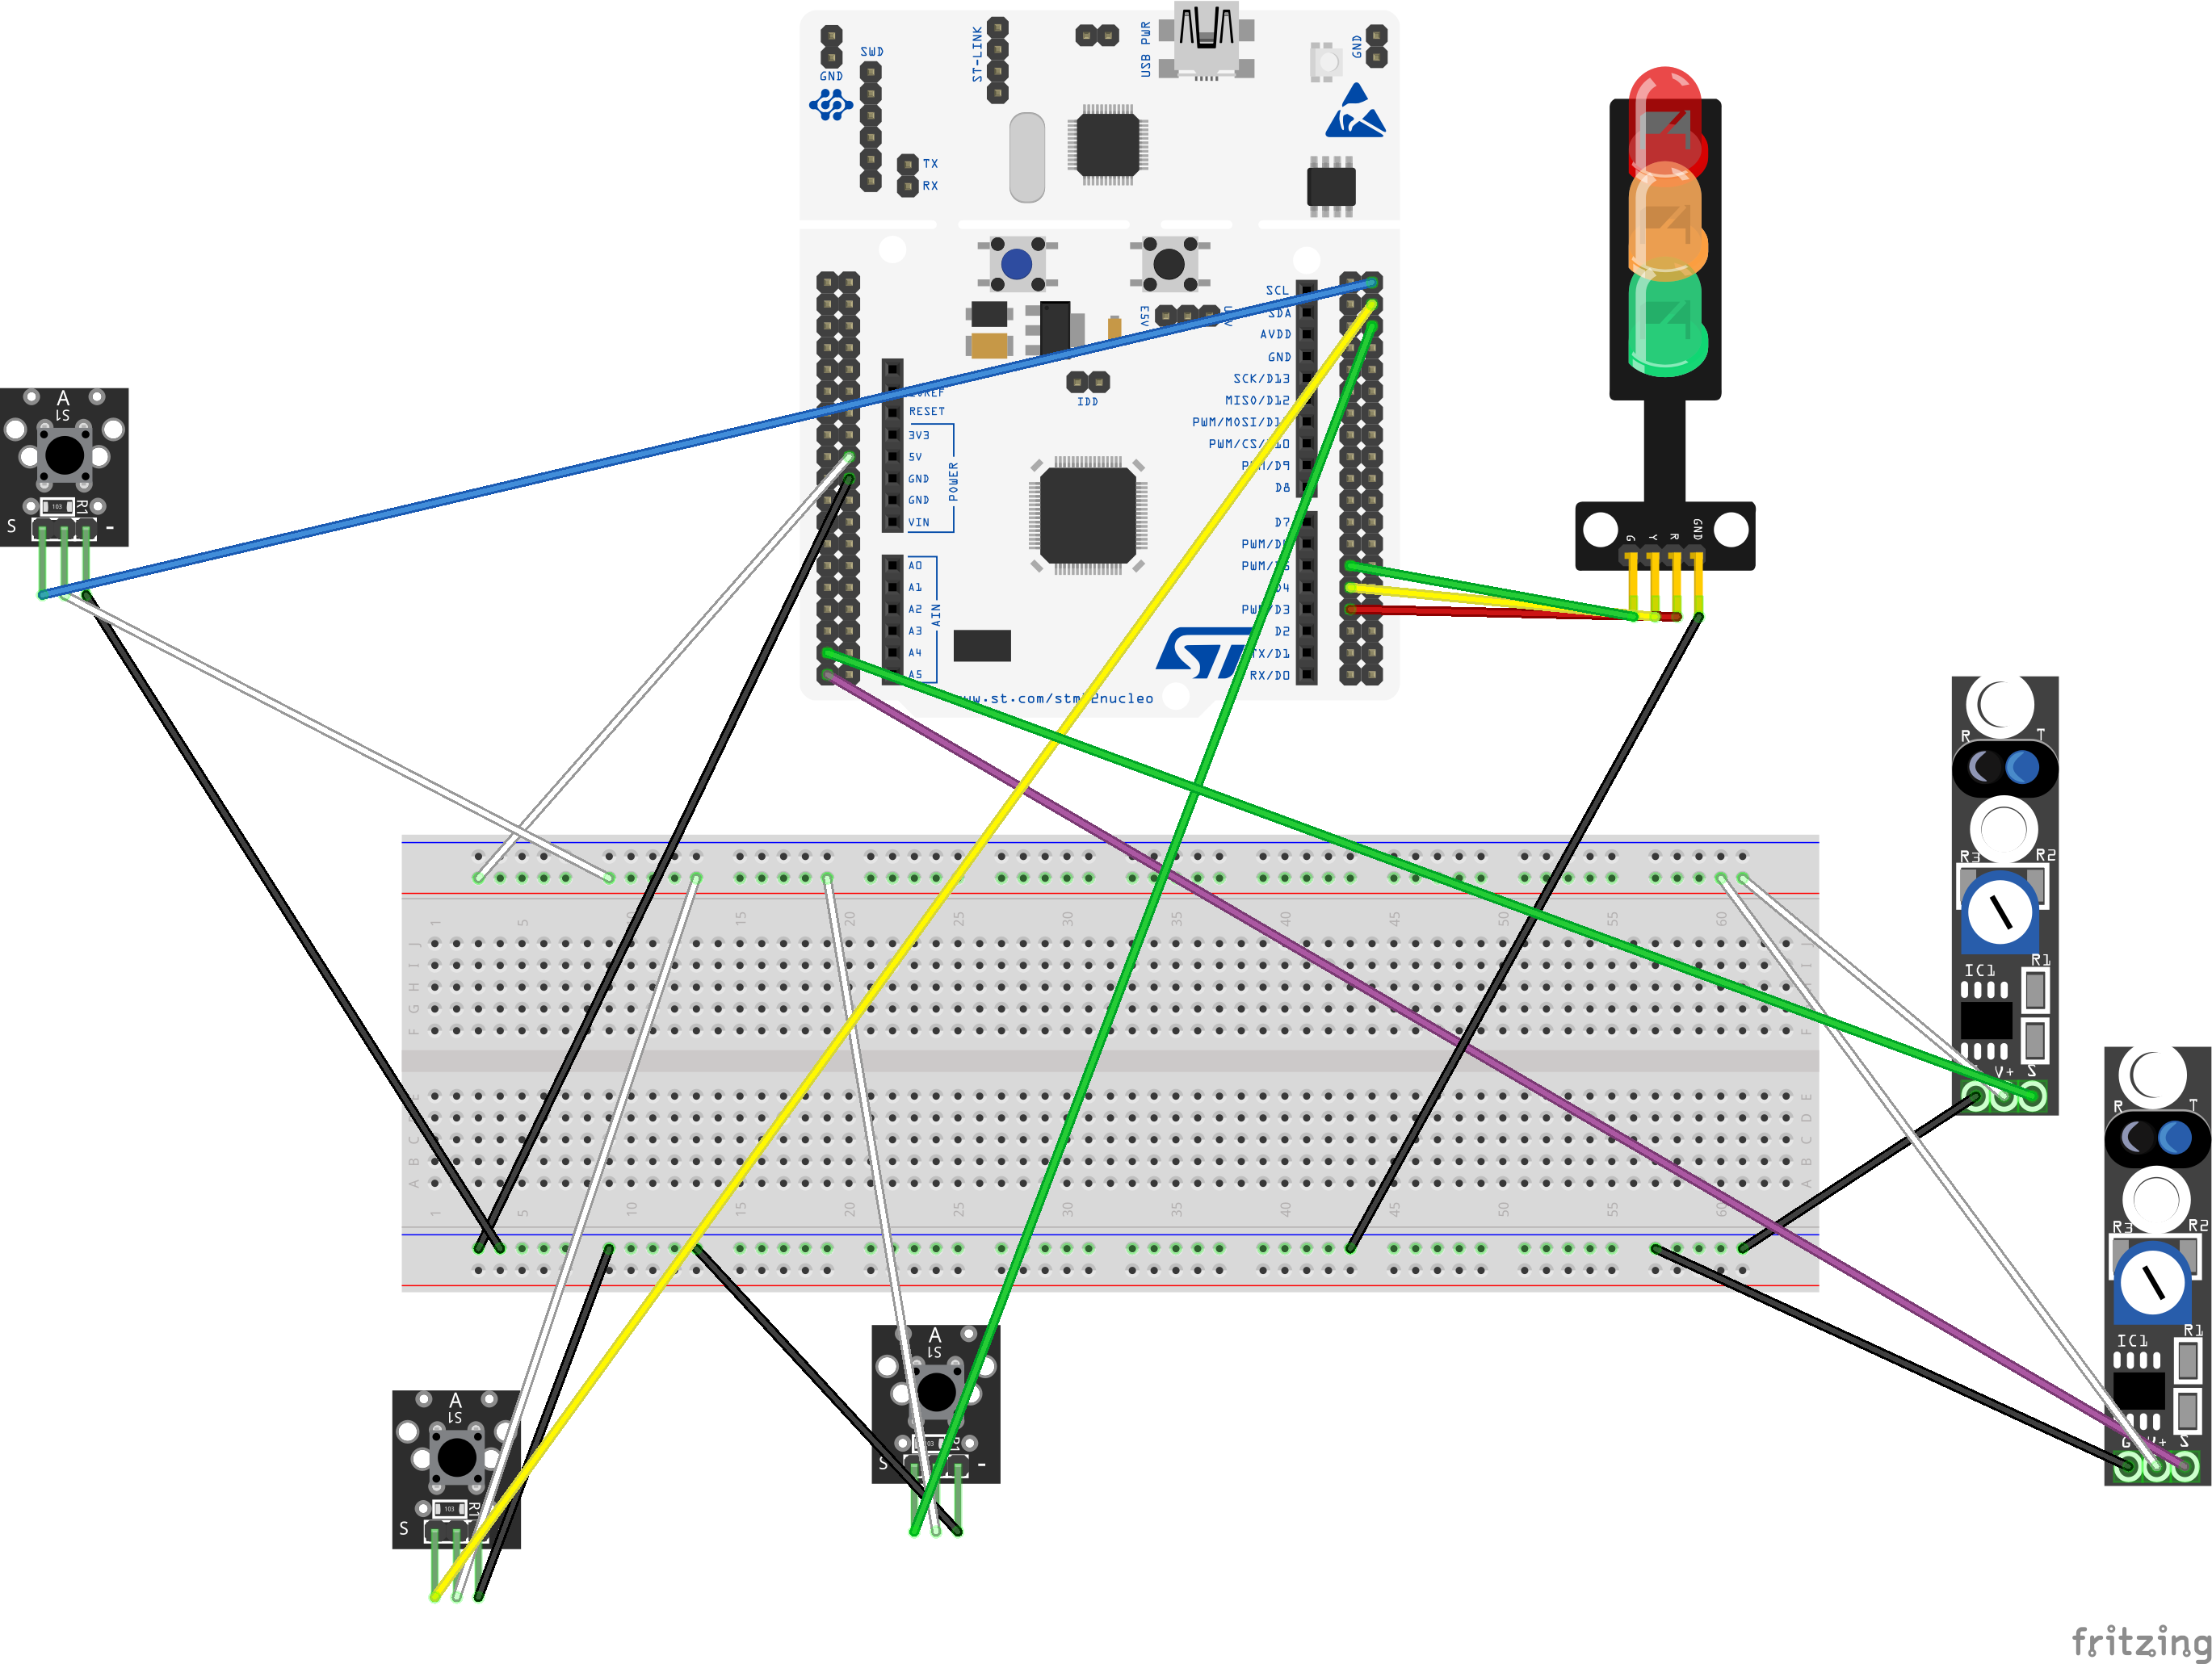
\includegraphics[width=0.9\textwidth]{figures/sketch_bb.png}
            \caption{Circuito su Fritzing}
            \label{sketch}
        \end{figure}


    \section{Codice Sorgente}
        Per generare il codice è stato utilizzato l'add-on \textbf{Embedded Coder}, il quale ha permesso la creazione di tutte le funzioni e variabili necessarie per realizzare l'automa. La creazione del codice sorgente tramite Embedded Coder è una metodologia avanzata che consente di generare codice C e C++ ottimizzato direttamente da modelli Simulink e Stateflow. Questo processo automatizzato non solo accelera lo sviluppo del software embedded, ma riduce anche la probabilità di errori manuali. Embedded Coder offre strumenti potenti per la configurazione del codice generato, permettendo di personalizzare le proprietà e le specifiche per soddisfare requisiti specifici dell'applicazione. Inoltre, supporta l'integrazione con ambienti di sviluppo integrato (IDE) e toolchain per microcontrollori, facilitando il deployment su hardware target.

        Il codice generato è stato importato nell'IDE \textbf{STM32CubeIDE}, dove è stato creato il file main per collegare i componenti fisici della scheda con le variabili create da MATLAB. Questo processo garantisce una sinergia ottimale tra il codice generato automaticamente e l'hardware, assicurando che tutti i sensori, attuatori e altri dispositivi siano correttamente interfacciati e operativi.

        \begin{listing}[!ht]
            \begin{minted}[breaklines=true]{c}
                #include "main.h"
                #include "gpio.h"
                #include "Chart.h"
                void SystemClock_Config(void);
                static void Chart_read_inputs(){
                    rtU.B1 = HAL_GPIO_ReadPin(B1_GPIO_Port, B1_Pin);
                    rtU.B2 = HAL_GPIO_ReadPin(B2_GPIO_Port, B2_Pin);
                    rtU.B3 = HAL_GPIO_ReadPin(B3_GPIO_Port, B3_Pin);
                    rtU.P1 = !HAL_GPIO_ReadPin(P1_GPIO_Port, P1_Pin);
                    rtU.P2 = !HAL_GPIO_ReadPin(P2_GPIO_Port, P2_Pin);
                }
                static void Chart_write_outputs(){
                    HAL_GPIO_WritePin(LedG_GPIO_Port, LedG_Pin, rtY.LedG);
                    HAL_GPIO_WritePin(LedY_GPIO_Port, LedY_Pin, rtY.LedY);
                    HAL_GPIO_WritePin(LedR_GPIO_Port, LedR_Pin, rtY.LedR);
                }
                int main(void)
                {
                    HAL_Init();
                    SystemClock_Config();
                    MX_GPIO_Init();
                    Chart_initialize();
                    while (1)
                    {
                        uint32_t elapsed, start;
                        start = HAL_GetTick();
                        Chart_read_inputs();
                        Chart_step();
                        Chart_write_outputs();
                        elapsed = HAL_GetTick() - start;
                        HAL_Delay(100-elapsed);
                    }
                    }
            \end{minted}
        \caption{Main}
    \label{listing:1}
\end{listing}